\documentclass{beamer}
\usepackage[utf8]{inputenc}
\usepackage[french]{babel}
\usepackage[T1]{fontenc}
\usepackage{verbatim}
\usepackage{beamerthemesplit}

\title{STIC-B-415 : La mouvance NoSQL}
\author{Laurent Contzen}
\date{\today}

\begin{document}

\frame{\titlepage}

\frame{\tableofcontents}


\section{Historique}
\begin{frame}
  \begin{center}
    \structure{\Huge \insertsection}
  \end{center}
\end{frame}

\frame{\frametitle{Historique}
  \begin{itemize}
  \item<1-> Les bases de données : un besoin fondamental
  \item<2-> Première standardisation : Codasyl Approach
  \item<3-> Le modèle relationnel
  \item<4-> Apparition de la mouvance NoSQL
  \end{itemize}
}

\section{Le modèle relationnel}
\begin{frame}
  \begin{center}
    \structure{\Huge \insertsection}
  \end{center}
\end{frame}

\frame{\frametitle{Le modèle relationnel : Structure}
  \begin{itemize}
  \item<1-> Données organisées sous forme de tables
  \item<2-> Schéma défini à l'avance
  \item<3-> Requêtes ou transactions en langage SQL
  \item<4-> Très formalisé
  \end{itemize}
}

\frame{\frametitle{Le modèle relationnel : Exemple de table}
  \begin{center}
    \begin{tabular}{| c | l | l | l | l |}
      \hline
      \textbf{\underline{Id}} & \textbf{Name} & \textbf{Show} & \textbf{Actor} \\
      \hline
      \hline
      1 & Jackson Teller & Sons of Anarchy & Charlie Hunnam \\
      \hline
      2 & John Dorian & Scrubs & Zach Braff  \\
      \hline
      3 & Bill Adama & Battlestar Galactica & Edward J. Olmos \\
      \hline
      4 & Kara Thrace & Battlestar Galactica & Katee Sackhoff \\
      \hline
      5 & Tyrion Lannister & Game of Thrones & Peter Dinklage \\
      \hline
      6 & Ted Mosby & How I Met Your Mother & Josh Radnor \\
      \hline
      7 & Seth Bullock & Deadwood & Timothy Oliphant \\
      \hline
      8 & Tobias Beecher & Oz & Lee Tergesen \\
      \hline
      9 & Emily Sullivan & Jericho & Ashley Scott \\
      \hline
      10 & Jimmy McNulty & The Wire & Dominic West \\
      \hline
    \end{tabular}
  \end{center} 
}

\frame{\frametitle{Le modèle relationnel : Exemples de requêtes SQL}
\begin{itemize}
\item<1-> SELECT * FROM Characters;
\item<2-> SELECT * FROM Characters WHERE Show=``Battlestar Galactica'';
\item<3-> SELECT Actor FROM Characters WHERE Name=''Tyrion Lannister'' AND Show=''Game of Thrones'';
\end{itemize}
}

\frame{\frametitle{Le modèle relationnel : Caractéristiques}
  \begin{itemize}
  \item<1-> Nécéssite beaucoup de rigueur
  \item<2-> Difficile de changer la structure une fois en utilisation
  \item<3-> Difficile à distribuer 
  \item<4-> Très peu de possibilités de redimmensionnement
  \end{itemize}
}

\section{ACID et CAP}
\begin{frame}
  \begin{center}
    \structure{\Huge \insertsection}
  \end{center}
\end{frame}

\frame{\frametitle{ACID}
  \begin{itemize}
  \item<1-> Atomicity : Reussite ou échec pour une transaction
  \item<2-> Consistency : Bases de données toujours dans un état correct
  \item<3-> Isolation : Transactions indépendantes et non simultanées 
  \item<4-> Durability : Pérénité des modifications
  \end{itemize}
}

\frame{\frametitle{CAP}
  \begin{itemize}
  \item<1-> Théorème CAP
  \item<2-> Consistency : Toujours accès à la dernière version de l'information
  \item<3-> Availability : La base de données est toujours en service et réponds toujours aux requêtes.
  \item<4-> Partition tolerance : Entièreté des données accessible même si une partie des serveurs tombe.
  \end{itemize}
}

\section{Différents cas d'utilisation}
\begin{frame}
  \begin{center}
    \structure{\Huge \insertsection}
  \end{center}
\end{frame}

\frame{\frametitle{Différents cas d'utilisation}
  \begin{itemize}
  \item<1-> Système bancaire
  \item<2-> Réseaux Sociaux
  \end{itemize}
}

\section{Les différents types de bases de données NoSQL}
\begin{frame}
  \begin{center}
    \structure{\Huge \insertsection}
  \end{center}
\end{frame}

\frame{\frametitle{Les différents types de bases de données NoSQL}
  \begin{center}
    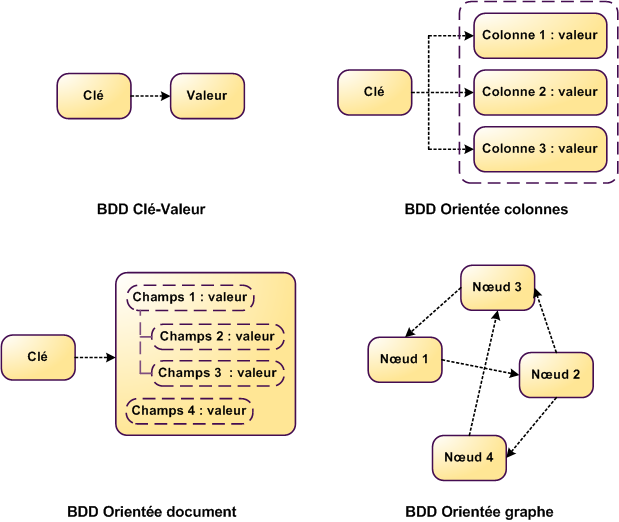
\includegraphics[width=\paperwidth,height=0.65\paperheight,keepaspectratio]{nosql.png}
  \end{center}
}

\subsection{Key-Value}
\begin{frame}
  \begin{center}
    \structure{\Huge \insertsubsection}
  \end{center}
\end{frame}

\frame{\frametitle{Les bases de données de type Key-Value}
  \begin{itemize}
  \item<1-> Grandes tables de hashage
  \item<2-> Lectures ou écritures à partir d'un identifiant
  \item<3-> Données en bloc binaire
  \item<4-> Table partitionnée répliquée
  \item<5-> Taux de consistance souhaité
  \item<6-> TODO : Rajouter exemple
  \end{itemize}
}

\subsection{Document-oriented}
\begin{frame}
  \begin{center}
    \structure{\Huge \insertsubsection}
  \end{center}
\end{frame}

\frame{\frametitle{Les bases de données orientées document}
  \begin{itemize}
  \item<1-> Extension du modèle Key-Value
  \item<2-> Données sous forme de document structuré
  \item<3-> Connaissance du contenu du document
  \item<4-> Possibilité de requêtes plus élaborées
  \end{itemize}
}

\subsection{Columns-oriented}
\begin{frame}
  \begin{center}
    \structure{\Huge \insertsubsection}
  \end{center}
\end{frame}

\frame{\frametitle{Les bases de données orientées colonnes}
  \begin{itemize}
  \item<1-> Extension du modèle Key-Value avec des principes du modèle relationnel
  \item<2-> Pour chaque clé, données sous forme de colonnes contenant les informations
  \item<3-> Uniquement les colonnes utiles pour chaque clé
  \end{itemize}
  \begin{center}
    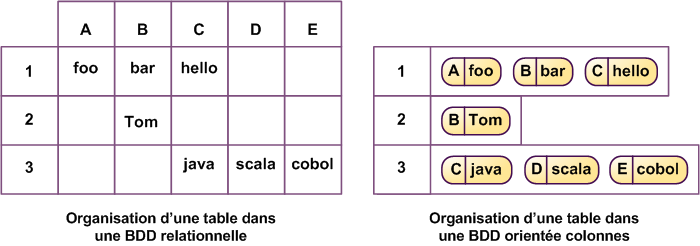
\includegraphics[width=0.3\paperwidth,height=0.3\paperheight,keepaspectratio]{nosql-colonnes.png}
  \end{center}
}

\subsection{Graph-oriented}
\begin{frame}
  \begin{center}
    \structure{\Huge \insertsubsection}
  \end{center}
\end{frame}



\end{document}
